\documentclass[aspectratio=169,11pt]{beamer}

%=====================================================
% Packages
%=====================================================

\usepackage{amsmath,amssymb}
\usepackage{graphicx}
\usepackage{booktabs}
\usepackage{array}
\usepackage{multicol}
\usepackage{mathtools}
\usepackage{tikz}
\usepackage{xcolor}

\usetikzlibrary{positioning,arrows.meta}

%=====================================================
% Theme
%=====================================================

\usetheme[numbering=fraction]{metropolis}

%=====================================================
% Colors
%=====================================================

\definecolor{Emerald}{RGB}{0,155,119}

\setbeamercolor{title}{fg=Emerald}

\setbeamercolor{frametitle}{
fg=white,
bg=Emerald
}

\setbeamercolor{progress bar}{
fg=Emerald
}

%=====================================================
% Remove Navigation Symbols
%=====================================================

\setbeamertemplate{navigation symbols}{}

%=====================================================
% Custom Frame Title
%=====================================================

\makeatletter

\setbeamertemplate{frametitle}
{
\nointerlineskip

\begin{beamercolorbox}[
wd=\paperwidth,
ht=3.6ex,
dp=1.4ex,
leftskip=0.6cm,
rightskip=0.6cm
]{frametitle}

\color{white}

\Large\bfseries

\makebox[\paperwidth-1.2cm][l]
{
\insertframetitle
\hfill
\normalsize\bfseries Arya T S
}

\end{beamercolorbox}
}

\makeatother

%=====================================================
% Information
%=====================================================

\title{Mathematics for Computing}

\subtitle{Assignment 01\\Sets and Relations}

\author{Arya T S}

\institute{
M.Tech Artificial Intelligence \& Software Engineering\\
Cochin University of Science and Technology (CUSAT)
}

\date{Semester I}

%=====================================================
% Document
%=====================================================

\begin{document}

%-----------------------------------------------------

\begin{frame}
\titlepage
\end{frame}

%-----------------------------------------------------

%=====================================================
\section{Sets}
%=====================================================

%-----------------------------------------------------
\begin{frame}{What is a Set?}

\begin{block}{Definition}

\vspace{0.1cm}

A \textbf{set} is a well-defined, unordered collection of distinct objects.
\end{block}

\vspace{0.3cm}

\textbf{Mathematical Representation}

\[
A=\{x\mid P(x)\}
\]

where \(P(x)\) is a predicate that determines whether
\(x\) belongs to the set.

\vspace{0.3cm}

\textbf{Example}
\[
F=\{\text{Age},\text{Income},\text{Experience},\text{Education}\}
\]

represents the feature set used to train a machine learning model.

\end{frame}

%-----------------------------------------------------

\begin{frame}{Representations of Sets}

A set can be represented in two standard forms.

\vspace{0.3cm}

\begin{columns}[T,onlytextwidth]

\column{0.49\textwidth}

\begin{block}{Roster Form}

Lists all elements of the set.

\begin{flushleft}
$\{1,2,3,4,5\}$
\end{flushleft}

\end{block}

\column{0.49\textwidth}

\begin{block}{Set Builder Form}

Defines the set using a common property.

\begin{flushleft}
$\{x\in\mathbb N \mid 1\le x\le5\}$
\end{flushleft}

\end{block}

\end{columns}

\vspace{0.5cm}

\[
\boxed{
\{1,2,3,4,5\}
=
\{x\in\mathbb N \mid 1\le x\le5\}
}
\]

\end{frame}

%=====================================================
\section{Set Builder Form}
%=====================================================

%-----------------------------------------------------
\begin{frame}{Set-Builder Form}

\begin{block}{Definition}

\vspace{0.1cm}

A set-builder form defines a set by specifying the
property satisfied by its elements.

\[
A=\{x\mid P(x)\}
\]

where \(P(x)\) is a predicate.

\end{block}

\vspace{0.4cm}

Instead of listing every element, we describe the
mathematical rule that generates the set or satisfies a condition.

\end{frame}

%-----------------------------------------------------

%-----------------------------------------------------
\begin{frame}{Examples (1--5)}

\small

\begin{enumerate}

\item $\{1,2,3,4,5,6,7\}
      =\{x\in\mathbb N\mid1\le x\le7\}$

\vspace{0.35cm}

\item $\{5,10,15,20,25\}
      =\{5n\mid1\le n\le5,\;n\in\mathbb N\}$

\vspace{0.35cm}

\item $\{3,6,9,12,15\}
      =\{3n\mid1\le n\le5,\;n\in\mathbb N\}$

\vspace{0.35cm}

\item $\{1,4,9,16,25,36\}
      =\{n^2\mid1\le n\le6,\;n\in\mathbb N\}$

\vspace{0.35cm}

\item $\{0,2,4,6,8\}
      =\{x\in\mathbb N\mid0\le x\le8,\;2\mid x\}$

\end{enumerate}

\end{frame}

%-----------------------------------------------------

%-----------------------------------------------------
\begin{frame}{Assignment Questions (6--10)}

\small

\begin{enumerate}
\setcounter{enumi}{5}

\item
$\left\{\frac{1}{2},\frac{2}{3},\frac{3}{4},\frac{4}{5},\frac{5}{6}\right\}
=
\left\{\frac{n}{n+1}\mid n\in\mathbb N,\;1\le n\le5\right\}$

\vspace{0.45cm}

\item
$\{2,4,8,16,32\}
=
\{2^n\mid n\in\mathbb N,\;1\le n\le5\}$

\vspace{0.45cm}

\item
$\{2,6,18,54,162\}
=
\{2\cdot3^n\mid n\in\mathbb N,\;0\le n\le4\}$

\vspace{0.45cm}

\item
$\{3,8,15,24,35,48\}
=
\{n^2-1\mid n\in\mathbb N,\;2\le n\le7\}$

\vspace{0.45cm}

\item
$\{2,3,5,7,11,13,17\}
=
\{x\in\mathbb N\mid x\ \text{is prime},\;x\le17\}$

\end{enumerate}

\end{frame}

%=====================================================
\section{Types of Sets}
%=====================================================

%-----------------------------------------------------
\begin{frame}{Cardinality and Finite Sets}

\begin{block}{Cardinality}

\[
|A|=\text{Number of elements in }A
\]

\textbf{Example:}
\[
A=\{2,4,6,8\}
\]
\[
|A|=4
\]

\end{block}

\vspace{0.1cm}

\begin{block}{Finite Set}

\[
|A|=n,\qquad n\in\mathbb N
\]
\textbf{Example:}
\[
Classes = \{\text{Cat},\text{Dog},\text{Bird}\} \]
\[|Classes| = 3
\]

\end{block}

\end{frame}

%=====================================================
\begin{frame}{Infinite and Null Sets}

\begin{block}{Infinite Set}

\[
|A|=\infty
\]

\textbf{Example:}
\[
\mathbb N=\{1,2,3,\ldots\}
\]

\end{block}

\vspace{0.1cm}

\begin{block}{Null (Empty) Set}

\[
A=\varnothing
\qquad\text{or}\qquad
|A|=0
\]

\textbf{Example:}
\[
\begin{aligned}
FP &= \varnothing
\end{aligned}
\]

\end{block}

\end{frame}

%=====================================================
\begin{frame}{Singleton and Equal Sets}

\begin{block}{Singleton Set}

\[
|A|=1
\]

\textbf{Example:}
\[
W=\{w^\ast\}
\]
where \(w^\ast\) is the unique optimal weight vector.

\end{block}

\vspace{0.1cm}

\begin{block}{Equal Sets}

\[
A=B
\iff
(\forall x)(x\in A\Leftrightarrow x\in B)
\]

\textbf{Example:}
\[
\{1,2,3\}=\{3,2,1\}
\]

\end{block}

\end{frame}

%=====================================================
\begin{frame}{Equivalent Sets and Subsets}

\begin{block}{Equivalent Sets}

\[
|A|=|B|
\]
\textbf{Example:}
\[
\begin{aligned}
|Training| &=1000\\
|Validation| &=1000
\end{aligned}
\]

\end{block}

\vspace{0.1cm}

\begin{block}{Subset}

\[
A\subseteq B
\]

\textbf{Example:}

\[
Dogs\subseteq Animals
\]

\end{block}

\end{frame}

%=====================================================
\begin{frame}{Superset and Universal Set}

\begin{block}{Superset}

\[
B\supseteq A
\]

\textbf{Example:}
\[
Animals\supseteq Dogs
\]

\end{block}

\vspace{0.1cm}

\begin{block}{Universal Set}

\[
U=\{\text{All Images}\}
\]

\textbf{Example:}

\[
Cats,\;Dogs,\;Cars\subseteq U
\]

\end{block}

\end{frame}

%=====================================================
\begin{frame}{Power Set and Countable Sets}

\begin{block}{Power Set}
\[
P(A)=\{X\mid X\subseteq A\}
\]
\textbf{Example:} 
\[
A=\{1,2\}\]
\[P(A)=\{\varnothing,\{1\},\{2\},\{1,2\}\}
\]

\end{block}

\vspace{0.1cm}

\begin{block}{Countable Set}

\[
f:\mathbb N\rightarrow A \;is \;a \;bijection.
\]

\textbf{Example:}
\[
\mathbb N,\;
\mathbb Z,\;
\mathbb Q
\;are \;countable, \;while\]
\[
\mathbb R\;
is\; uncountable.\]

\end{block}

\end{frame}

%=====================================================
\section{Set Operations}
%=====================================================


%-----------------------------------------------------
\begin{frame}{Set Operations}

\begin{block}{Definition}

\vspace{0.1cm}

Set operations combine or modify sets to create new sets.
\[
A,B \rightarrow \text{New Set}
\]

\end{block}

\vspace{0.1cm}

Common set operations:

\begin{enumerate}
    \item Union
    \item Intersection
    \item Set Difference
    \item Symmetric Difference
    \item Complement
    \item Cartesian Product
\end{enumerate}


\end{frame}


%-----------------------------------------------------
\begin{frame}{Union of Sets}

\begin{block}{Mathematical Definition}

\vspace{0.1cm}

The union of two sets contains all the elements that belong
to either set.

\[
A\cup B=\{x\mid x\in A\lor x\in B\}
\]

\end{block}

\vspace{0.1cm}

Example:
\[
A=\{1,2,3\}
\]
\[
B=\{3,4,5\}
\]
\[
A\cup B=\{1,2,3,4,5\}
\]

Example:
Combining two feature sets from different datasets.
\[
Features =
A\cup B
\]

\end{frame}

%-----------------------------------------------------
\begin{frame}{Intersection of Sets}

\begin{block}{Mathematical Definition}

\vspace{0.1cm}

The intersection contains elements common to both sets.

\[
A\cap B=\{x\mid x\in A\land x\in B\}
\]

\end{block}

Example:
\[
A=\{Python,Java,C++\}
\]
\[
B=\{Python,R,Java\}
\]
\[
A\cap B=\{Python,Java\}
\]

Example:
Common features selected by two machine learning models.
\[
Selected=A\cap B
\]

\end{frame}



%-----------------------------------------------------
\begin{frame}{Set Difference}

\begin{block}{Mathematical Definition}

\vspace{0.1cm}

The difference of two sets contains elements present in
one set, but not in the other.

\[
A-B=\{x\mid x\in A\land x\notin B\}
\]

\end{block}

Example:
\[
A=\{1,2,3,4,5\}
\]
\[
B=\{3,4,5,6,7\}
\]
\[
A-B=\{1,2\}
\]

Example:
Removing already processed data samples:
\[
NewData=Dataset-Processed
\]

\end{frame}

%-----------------------------------------------------
\begin{frame}{Symmetric Difference}

\begin{block}{Mathematical Definition}

\vspace{0.1cm}

The symmetric difference contains elements that belong
to exactly one of the sets.

\[
A\triangle B=(A-B)\cup(B-A)
\]

\end{block}

Example:
\[
A=\{1,2,3\}
\]
\[
B=\{3,4,5\}
\]
\[
A\triangle B=\{1,2,4,5\}
\]

Example:
Files modified in either branch but not both.
\[
Changes=A\triangle B
\]

\end{frame}

%-----------------------------------------------------
\begin{frame}{Complement of a Set}

\begin{block}{Mathematical Definition}

\vspace{0.1cm}

The complement contains elements from the universal set
that are not present in the given set.
\[
A^c=U-A
\]

\end{block}

Example:
\[
U=\{1,2,3,4,5\}
\]
\[
A=\{1,2\}
\]
\[
A^c=\{3,4,5\}
\]

Example:
Classification errors:
\[
Correct^c = Incorrect
\]

\end{frame}

%-----------------------------------------------------
\begin{frame}{Cartesian Product}

\begin{block}{Mathematical Definition}

\vspace{0.1cm}

Cartesian product creates ordered pairs.
\[
A\times B=
\{(a,b)\mid a\in A,\ b\in B\}
\]

\end{block}
Example:
\[
A=\{1,2\}
\]
\[
B=\{Python,Java\}
\]
\[
A\times B=
\{
(1,Python),
(1,Java),
(2,Python),
(2,Java)
\}
\]

Example:
Input-output pairs in supervised learning:
\[
(X,Y)\;where
\]
\[
X\times Y\;represents \;possible\; input-label\; combinations.
\]

\end{frame}

%-----------------------------------------------------
\begin{frame}{Set Operations using Venn Diagrams}

\begin{center}
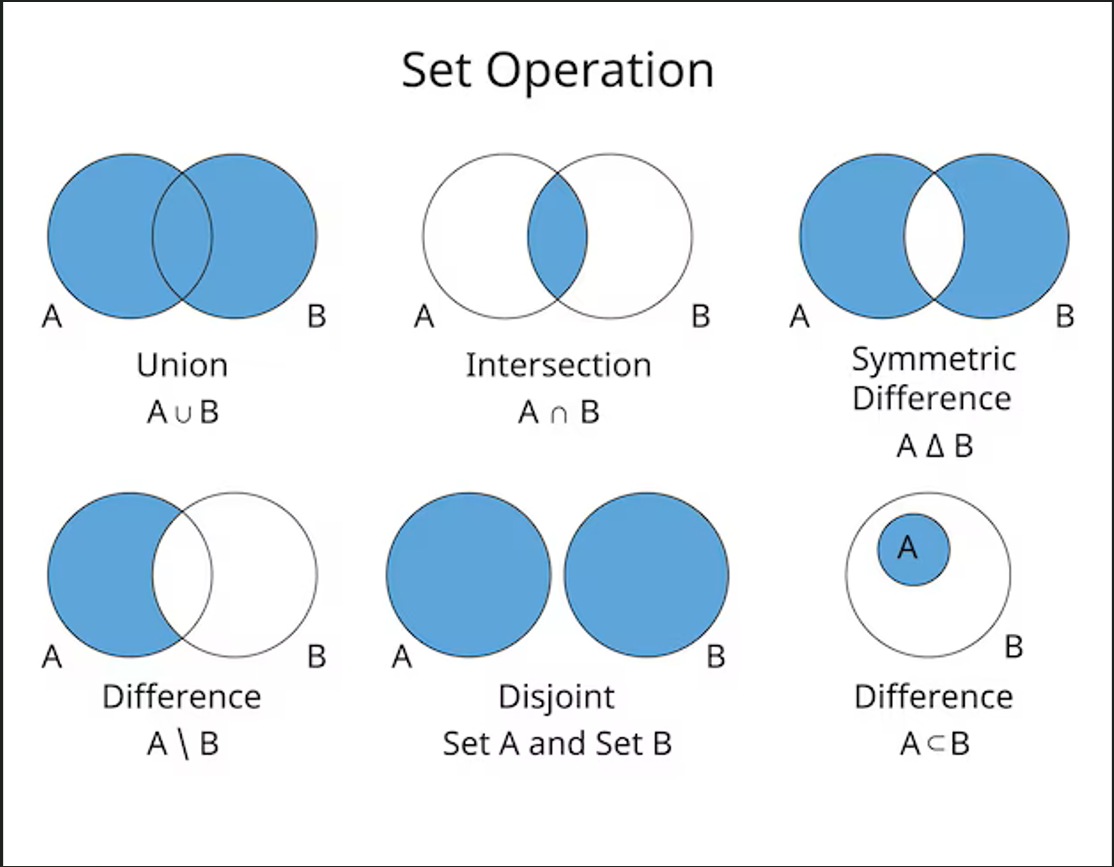
\includegraphics[width=0.7\linewidth]{images/operations.png}
\end{center}

\end{frame}

%=====================================================
\section{Inclusion-Exclusion Principle}
%=====================================================

%-----------------------------------------------------
\begin{frame}{Inclusion-Exclusion Principle}

\textbf{Definition}

\vspace{0.3cm}

The Inclusion-Exclusion Principle is used to determine the
cardinality of the union of overlapping sets without counting
common elements more than once.

\vspace{0.5cm}

For two finite sets,

\[
|A\cup B|
=
|A|
+
|B|
-
|A\cap B|
\]

\end{frame}

%-----------------------------------------------------

\begin{frame}{Example:}

Suppose an autonomous driving model detects
\[
A=
\{\text{Pixels predicted as Road}\}
\]
\[
B=
\{\text{Ground Truth Road Pixels}\}
\]

Suppose
\[
|A|=1200
\]
\[
|B|=1100
\]
\[
|A\cap B|=950
\]
Then
\[
|A\cup B|
=
1200+1100-950
=
1350
\]

The union represents all pixels that are
either predicted as road or actually belong
to the road region.

\end{frame}

%-----------------------------------------------------
\begin{frame}{General Inclusion-Exclusion Formula}

For \(n\) finite sets,

\vspace{0.3cm}

\[
\left|
\bigcup_{i=1}^{n}
A_i
\right|
=
\sum |A_i|
-
\sum |A_i\cap A_j|
+
\sum |A_i\cap A_j\cap A_k|
-\cdots
+(-1)^{n+1}
\left|
\bigcap_{i=1}^{n}
A_i
\right|
\]

\end{frame}

%=====================================================
\section{Relations}
%=====================================================

%-----------------------------------------------------
\begin{frame}{Binary Relation}

\textbf{Definition}

A binary relation from $A$ to $B$ is any subset of

\[
A\times B
\]

Mathematically,
\[
R\subseteq A\times B \;if \;(a,b)\in R\]
We write aRb meaning "$a$ is related to $b$."

\end{frame}

%-----------------------------------------------------

\begin{frame}{Example of a Binary Relation}

Let
\[
A=\{1,2,3\}
\]

Define
\[
R=
\{
(1,2),
(2,3),
(1,3)
\}
\]

Then
\[
R\subseteq A\times A
\]

Hence,
\[
R\;is\; a\; binary\; relation\; on\; A.
\]

\end{frame}

%-----------------------------------------------------

\begin{frame}{Predicate Representation}

A relation is often defined using a predicate.

\vspace{0.4cm}

Example

\[
R=
\{
(a,b)
\mid
a,b\in A
\land
a<b
\}
\]

where

\[
P(a,b):a<b
\]

is the predicate.

\end{frame}

%-----------------------------------------------------

\begin{frame}{Domain and Range of a Relation}

For

\[
R\subseteq A\times B
\]

the \textbf{Domain} is

\[
Dom(R)
=
\{
a\in A
\mid
\exists b\in B,
(a,b)\in R
\}
\]

The \textbf{Range} is

\[
Ran(R)
=
\{
b\in B
\mid
\exists a\in A,
(a,b)\in R
\}
\]

\end{frame}

%=====================================================
\section{Properties of Relations}
%=====================================================

%-----------------------------------------------------
\begin{frame}{Properties of Relations}

The six fundamental properties are

\begin{itemize}
    \item Reflexive
    \item Irreflexive
    \item Symmetric
    \item Antisymmetric
    \item Asymmetric
    \item Transitive
\end{itemize}

These properties help determine whether a relation is an Equivalence Relation or a Partial Order.

\end{frame}

%-----------------------------------------------------

\begin{frame}{Reflexive and Irreflexive Relations}

\begin{columns}

\column{0.48\textwidth}

\textbf{Reflexive}

\vspace{0.1cm}

$\forall a\in A,\;(a,a)\in R$

Every element is related to itself.

\vspace{0.3cm}

Example:

$\le,\quad =,\quad \subseteq$

\column{0.48\textwidth}

\textbf{Irreflexive}

\vspace{0.1cm}

$\forall a\in A,\;
(a,a)\notin R$

No element is related to itself.

\vspace{0.3cm}

Example:

$<,\quad >$

\end{columns}

\end{frame}

%-----------------------------------------------------

\begin{frame}{Symmetric Relation}

\textbf{Definition}

\[
(a,b)\in R
\Longrightarrow
(b,a)\in R
\]

\vspace{0.5cm}

Example:

\[
xRy
\iff
x
\text{ and }
y
\text{ belong to the same class}
\]

\[
(Student_1,Student_2)
\Longrightarrow
(Student_2,Student_1)
\]

\end{frame}

%-----------------------------------------------------

\begin{frame}{Antisymmetric Relation}

\textbf{Definition}

\[
(a,b)\in R
\land
(b,a)\in R
\Longrightarrow
a=b
\]

\vspace{0.5cm}

Example:
\[
\subseteq
\]
If
\[
A\subseteq B
\; and\;
B\subseteq A
\]
then
\[
A=B
\]

\end{frame}

%-----------------------------------------------------

\begin{frame}{Asymmetric Relation}

\textbf{Definition}

\[
(a,b)\in R
\Longrightarrow
(b,a)\notin R
\]

\vspace{0.4cm}

Example:
\[
<
\]
If
\[
3<5
\]
then
\[
5<3
\]

is false.

\end{frame}

%-----------------------------------------------------

\begin{frame}{Transitive Relation}

\textbf{Definition}

\[
(a,b)\in R
\land
(b,c)\in R
\Longrightarrow
(a,c)\in R
\]

\vspace{0.5cm}

Example:

\[
\le,\quad \subseteq
\]

\end{frame}

%-----------------------------------------------------

\begin{frame}{Applications in AI \& Software Engineering}

\begin{block}{Software Dependency Graph}

\vspace{0.1cm}

If
\[
Module_A
\rightarrow
Module_B
\]
and
\[
Module_B
\rightarrow
Module_C
\]
then
\[
Module_A
\]
indirectly depends on
\[
Module_C
\]
illustrating transitivity.

\end{block}

\end{frame}

%=====================================================
\section{Equivalence Relations and Partial Orders}
%=====================================================

%-----------------------------------------------------
\begin{frame}{Equivalence Relation}

\begin{block}{Definition}

\vspace{0.1cm}

A relation $R$ on a set $A$ is called an \textbf{Equivalence Relation} if

\[
R
\text{ is }
\boxed{\text{Reflexive}}
\land
\boxed{\text{Symmetric}}
\land
\boxed{\text{Transitive}}
\]

\end{block}

\end{frame}

%-----------------------------------------------------

\begin{frame}{Application of Equivalence Relations}

Suppose an image classifier predicts

\[
Images=
\{
Dog_1,
Dog_2,
Dog_3,
Cat_1,
Cat_2,
Car_1
\}
\]

Define
\[
xRy
\iff
\text{$x$ and $y$ belong to the same class}
\]

Equivalence Classes

\[
Dogs=
\{Dog_1,Dog_2,Dog_3\}
\]
\[
Cats=
\{Cat_1,Cat_2\}
\]
\[
Cars=
\{Car_1\}
\]

\end{frame}

%-----------------------------------------------------


%=====================================================
\section{Partially Ordered Sets}
%=====================================================

%-----------------------------------------------------

\begin{frame}{Partial Order}

\begin{block}{Definition}

\vspace{0.1cm}

A relation $R$ on a set $A$ is called a \textbf{Partial Order} if

\[
R
\text{ is }
\boxed{\text{Reflexive}}
\land
\boxed{\text{Antisymmetric}}
\land
\boxed{\text{Transitive}}
\]

\end{block}

\vspace{0.3cm}

A set together with a partial order,
\[
(A,R)
\]
is called a
\[
\boxed{\textbf{Partially Ordered Set (Poset)}}
\]

\end{frame}

%-----------------------------------------------------

\begin{frame}{Power Set as a Poset}

Let
\[
A=\{1,2,3\}
\]
Its power set is
\[
\mathcal P(A)
=
\{
\emptyset,
\{1\},
\{2\},
\{3\},
\{1,2\},
\{1,3\},
\{2,3\},
\{1,2,3\}
\}
\]
Define
\[
R=\subseteq
\]
Then
\[
(\mathcal P(A),\subseteq)
\]
is a Partially Ordered Set.

\end{frame}

%-----------------------------------------------------

\begin{frame}{Application}

A software project contains the tasks
\[
Collect
\rightarrow
Design
\rightarrow
Develop
\rightarrow
Test
\rightarrow
Deploy
\]

Define
\[
A\le B
\]
to mean
\[
\text{Task }A
\text{ must be completed before Task }B.
\]

This dependency relation is
\begin{itemize}
\item Reflexive
\item Antisymmetric
\item Transitive
\end{itemize}
Hence, it forms a Partial Order.

\end{frame}

%=====================================================
\section{Hasse Diagrams}
%=====================================================

\begin{frame}{Hasse Diagram}

\textbf{Definition}

A \textbf{Hasse Diagram} is a graphical representation of a partially
ordered set (poset), obtained by removing self-loops, arrowheads and
transitive edges.

\vspace{0.8cm}

\begin{block}{Purpose}

\vspace{0.1cm}
 It provides a simplified visualization of the ordering relationship between the elements of a poset.
\end{block}

\end{frame}

%=====================================================

\begin{frame}{Hasse Diagram of $\left(\mathcal P(A),\subseteq\right)$}

Let
\[
A=\{1,2\}
\]
Then
\[
\mathcal P(A)=
\left\{
\emptyset,\,
\{1\},\,
\{2\},\,
\{1,2\}
\right\}
\]
with the partial order
\[
R=\subseteq .
\]

\begin{columns}

\column{0.45\textwidth}

\centering

\begin{tikzpicture}[scale=1.1]

\node (e) at (0,0) {$\emptyset$};

\node (1) at (-1.2,1.5) {$\{1\}$};
\node (2) at (1.2,1.5) {$\{2\}$};

\node (12) at (0,3) {$\{1,2\}$};

\draw (e)--(1);
\draw (e)--(2);
\draw (1)--(12);
\draw (2)--(12);

\end{tikzpicture}

\column{0.55\textwidth}

\textbf{Observation}

\begin{itemize}
\item $\emptyset$ is the least element.
\item $\{1,2\}$ is the greatest element.
\item $\{1\}$ and $\{2\}$ are incomparable.
\item This is a partially ordered set.
\end{itemize}

\end{columns}

\end{frame}

%=====================================================
\begin{frame}{Hasse Diagram of $\left(\mathcal P(A),\subseteq\right)$}
\[Let\;
A=\{1,2,3\},
S=\mathcal P(A),
R=\subseteq.
\; Then,\;
(S,R)
\; is\; a\; partially\;ordered\;set\]
\centering

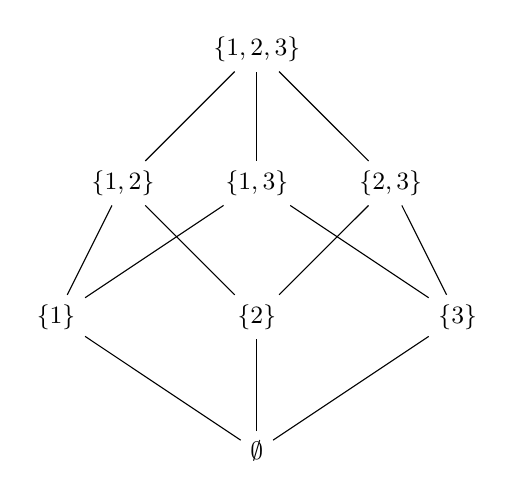
\begin{tikzpicture}[
    scale=0.85,
    every node/.style={font=\small}
]

% Bottom
\node (e) at (0,0) {$\emptyset$};

% Level 1
\node (1) at (-3,2) {$\{1\}$};
\node (2) at (0,2) {$\{2\}$};
\node (3) at (3,2) {$\{3\}$};

% Level 2
\node (12) at (-2,4) {$\{1,2\}$};
\node (13) at (0,4) {$\{1,3\}$};
\node (23) at (2,4) {$\{2,3\}$};

% Top
\node (123) at (0,6) {$\{1,2,3\}$};

% Edges
\draw (e)--(1);
\draw (e)--(2);
\draw (e)--(3);

\draw (1)--(12);
\draw (1)--(13);

\draw (2)--(12);
\draw (2)--(23);

\draw (3)--(13);
\draw (3)--(23);

\draw (12)--(123);
\draw (13)--(123);
\draw (23)--(123);

\end{tikzpicture}

\end{frame}

%=====================================================
\section{Maximum, Minimum, Chain and Antichain}
%=====================================================

%-----------------------------------------------------
\begin{frame}{Maximum and Minimum Elements}

\textbf{Let } $(P,\leq)$ \textbf{ be a partially ordered set.}

\vspace{0.5cm}

\begin{block}{Maximum Element}

\vspace{0.1cm}

An element $m\in P$ is called the \textbf{maximum (greatest)} element if

\[
\forall x\in P,\; x\leq m.
\]

\end{block}

\vspace{0.4cm}

\begin{block}{Minimum Element}

\vspace{0.1cm}

An element $n\in P$ is called the \textbf{minimum (least)} element if

\[
\forall x\in P,\; n\leq x.
\]

\end{block}

\end{frame}

%-----------------------------------------------------

\begin{frame}{Example using a Hasse Diagram}

\centering

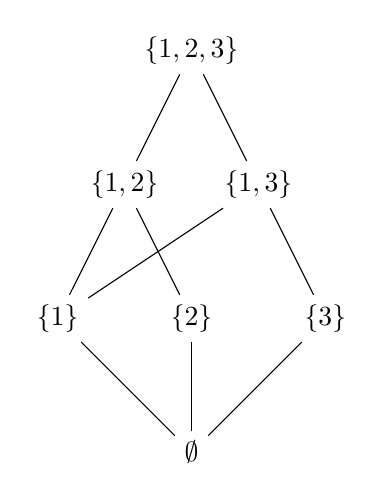
\begin{tikzpicture}[scale=0.85]

\node (a) at (0,0) {$\emptyset$};

\node (b) at (-2,2) {$\{1\}$};
\node (c) at (0,2) {$\{2\}$};
\node (d) at (2,2) {$\{3\}$};

\node (e) at (-1,4) {$\{1,2\}$};
\node (f) at (1,4) {$\{1,3\}$};

\node (g) at (0,6) {$\{1,2,3\}$};

\draw (a)--(b);
\draw (a)--(c);
\draw (a)--(d);

\draw (b)--(e);
\draw (b)--(f);

\draw (c)--(e);

\draw (d)--(f);

\draw (e)--(g);
\draw (f)--(g);

\end{tikzpicture}
\[
\boxed{
\begin{aligned}
\text{Minimum Element} &= \emptyset\\
\text{Maximum Element} &= \{1,2,3\}
\end{aligned}
}
\]

\end{frame}

%-----------------------------------------------------

\begin{frame}{Chain and Antichain}

\begin{block}{Chain}

A \textbf{chain} is a subset of a poset in which every pair of
elements is comparable.
\[
\forall a,b\in C,\;
a\leq b
\;\text{or}\;
b\leq a.
\]
Example:
\[
\emptyset
\subseteq
\{1\}
\subseteq
\{1,2\}
\subseteq
\{1,2,3\}
\]

\end{block}

\begin{block}{Antichain}

An \textbf{antichain} is a subset in which no two distinct
elements are comparable.
\[
\forall a\neq b,\;
a\nleq b
\land
b\nleq a.
\]
Example: 
\[
\{\{1\},\{2\},\{3\}\}
\]

\end{block}

\end{frame}

%-----------------------------------------------------

\begin{frame}[standout]
\Huge
Thank You
\end{frame}

\end{document}